\documentclass{beamer}
\usepackage{graphicx, subfigure}

\usetheme[compress]{Dresden}
\setbeamertemplate{navigation symbols}{} 

\title{Locate My Plate \\ A License Plate Localisation System}
\subtitle{presented by: Tjerk Kostelijk, Folkert Huizinga}
\date{July 1, 2009}

\begin{document}

\frame{\titlepage}

\setcounter{tocdepth}{1}

\frame
{
  \frametitle{Outline}
  \small
  \tableofcontents
  \normalsize
}

\setcounter{tocdepth}{2}

\section{Introduction}
\frame
{
  \frametitle{Introduction}
	
  \begin{itemize}
  \item <+-| alert@+> Implementation License Plate Localisation
  \item <+-| alert@+> Feature Analysis
  \item <+-| alert@+> Cascading Classifier
  \item <+-| alert@+> Strong Classifier
  \item <+-| alert@+> Weak Classifier
  \end{itemize}
}

\section{Features}
\frame
{
  \frametitle{Features}
	
  \begin{itemize}
  \item <+-| alert@+> Image Filter
  \item <+-| alert@+> Image Type
  \item <+-| alert@+> Horizontal or Vertical
  \item <+-| alert@+> Generation using powerset
  \end{itemize}
}

\frame
{
	\begin{figure}[!ht]
		\centering
		\subfigure{
		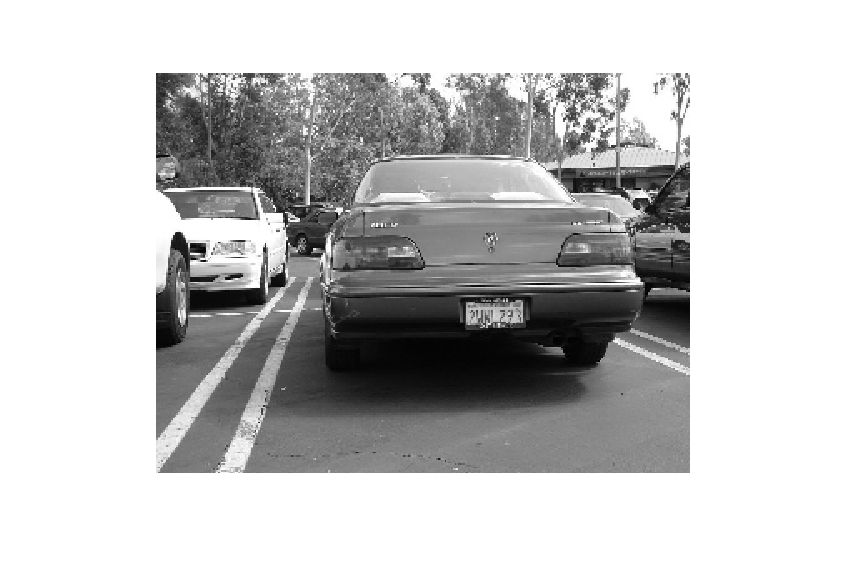
\includegraphics[height=3.5cm]{../report/img/original}
		\label{fig:a}
		}
		\subfigure{
		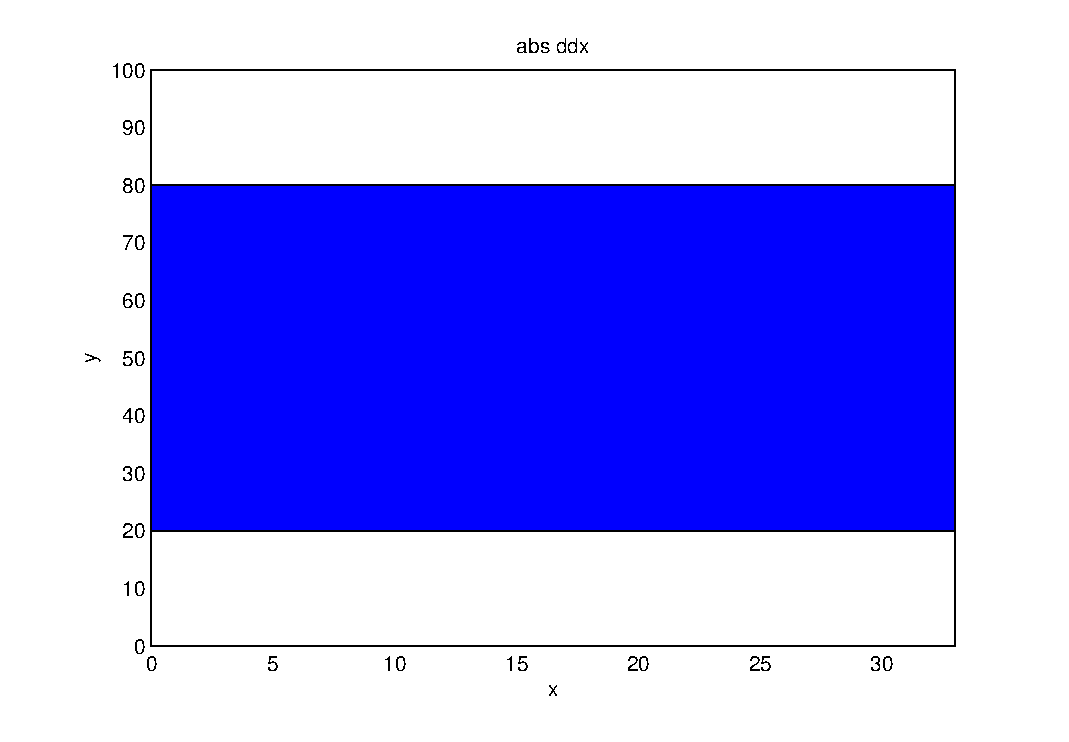
\includegraphics[height=3.5cm]{../report/img/feature}
		\label{fig:b}
		}
		\subfigure{
		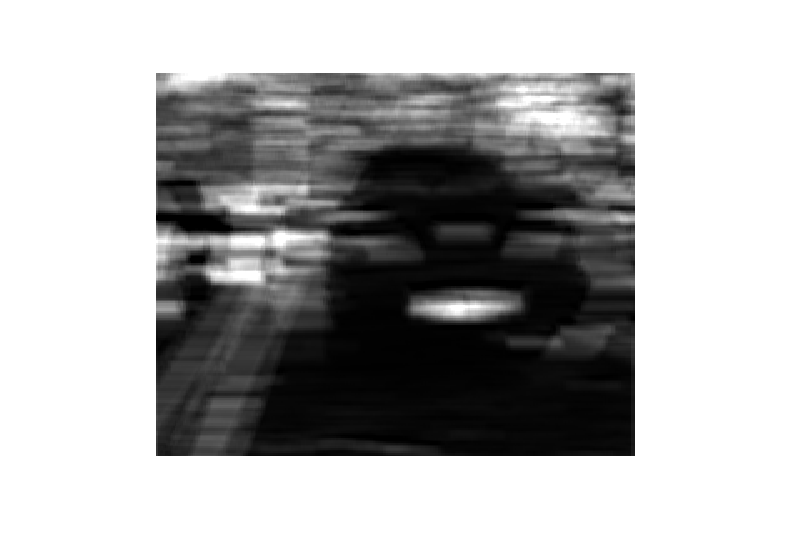
\includegraphics[height=3.5cm]{../report/img/featureapplied}
		\label{fig:c}
		}
		\caption{A horizontal, second order $x$-derivative feature with binary code
		$01110$, consisting of three blocks applied to an image.}
		\label{fig:feature}
	\end{figure}
}

\section{Stage I: Weak}
\frame
{
  \frametitle{Stage I: Weak}
	
  \begin{itemize}
  \item <+-| alert@+> xxx
  \end{itemize}
}

\section{Stage II: Strong}
\frame
{
  \frametitle{Stage II: Strong}
	
  \begin{itemize}
  \item <+-| alert@+> xxx
  \end{itemize}
}

\frame
{
	\begin{figure}[!ht]
	\centering
	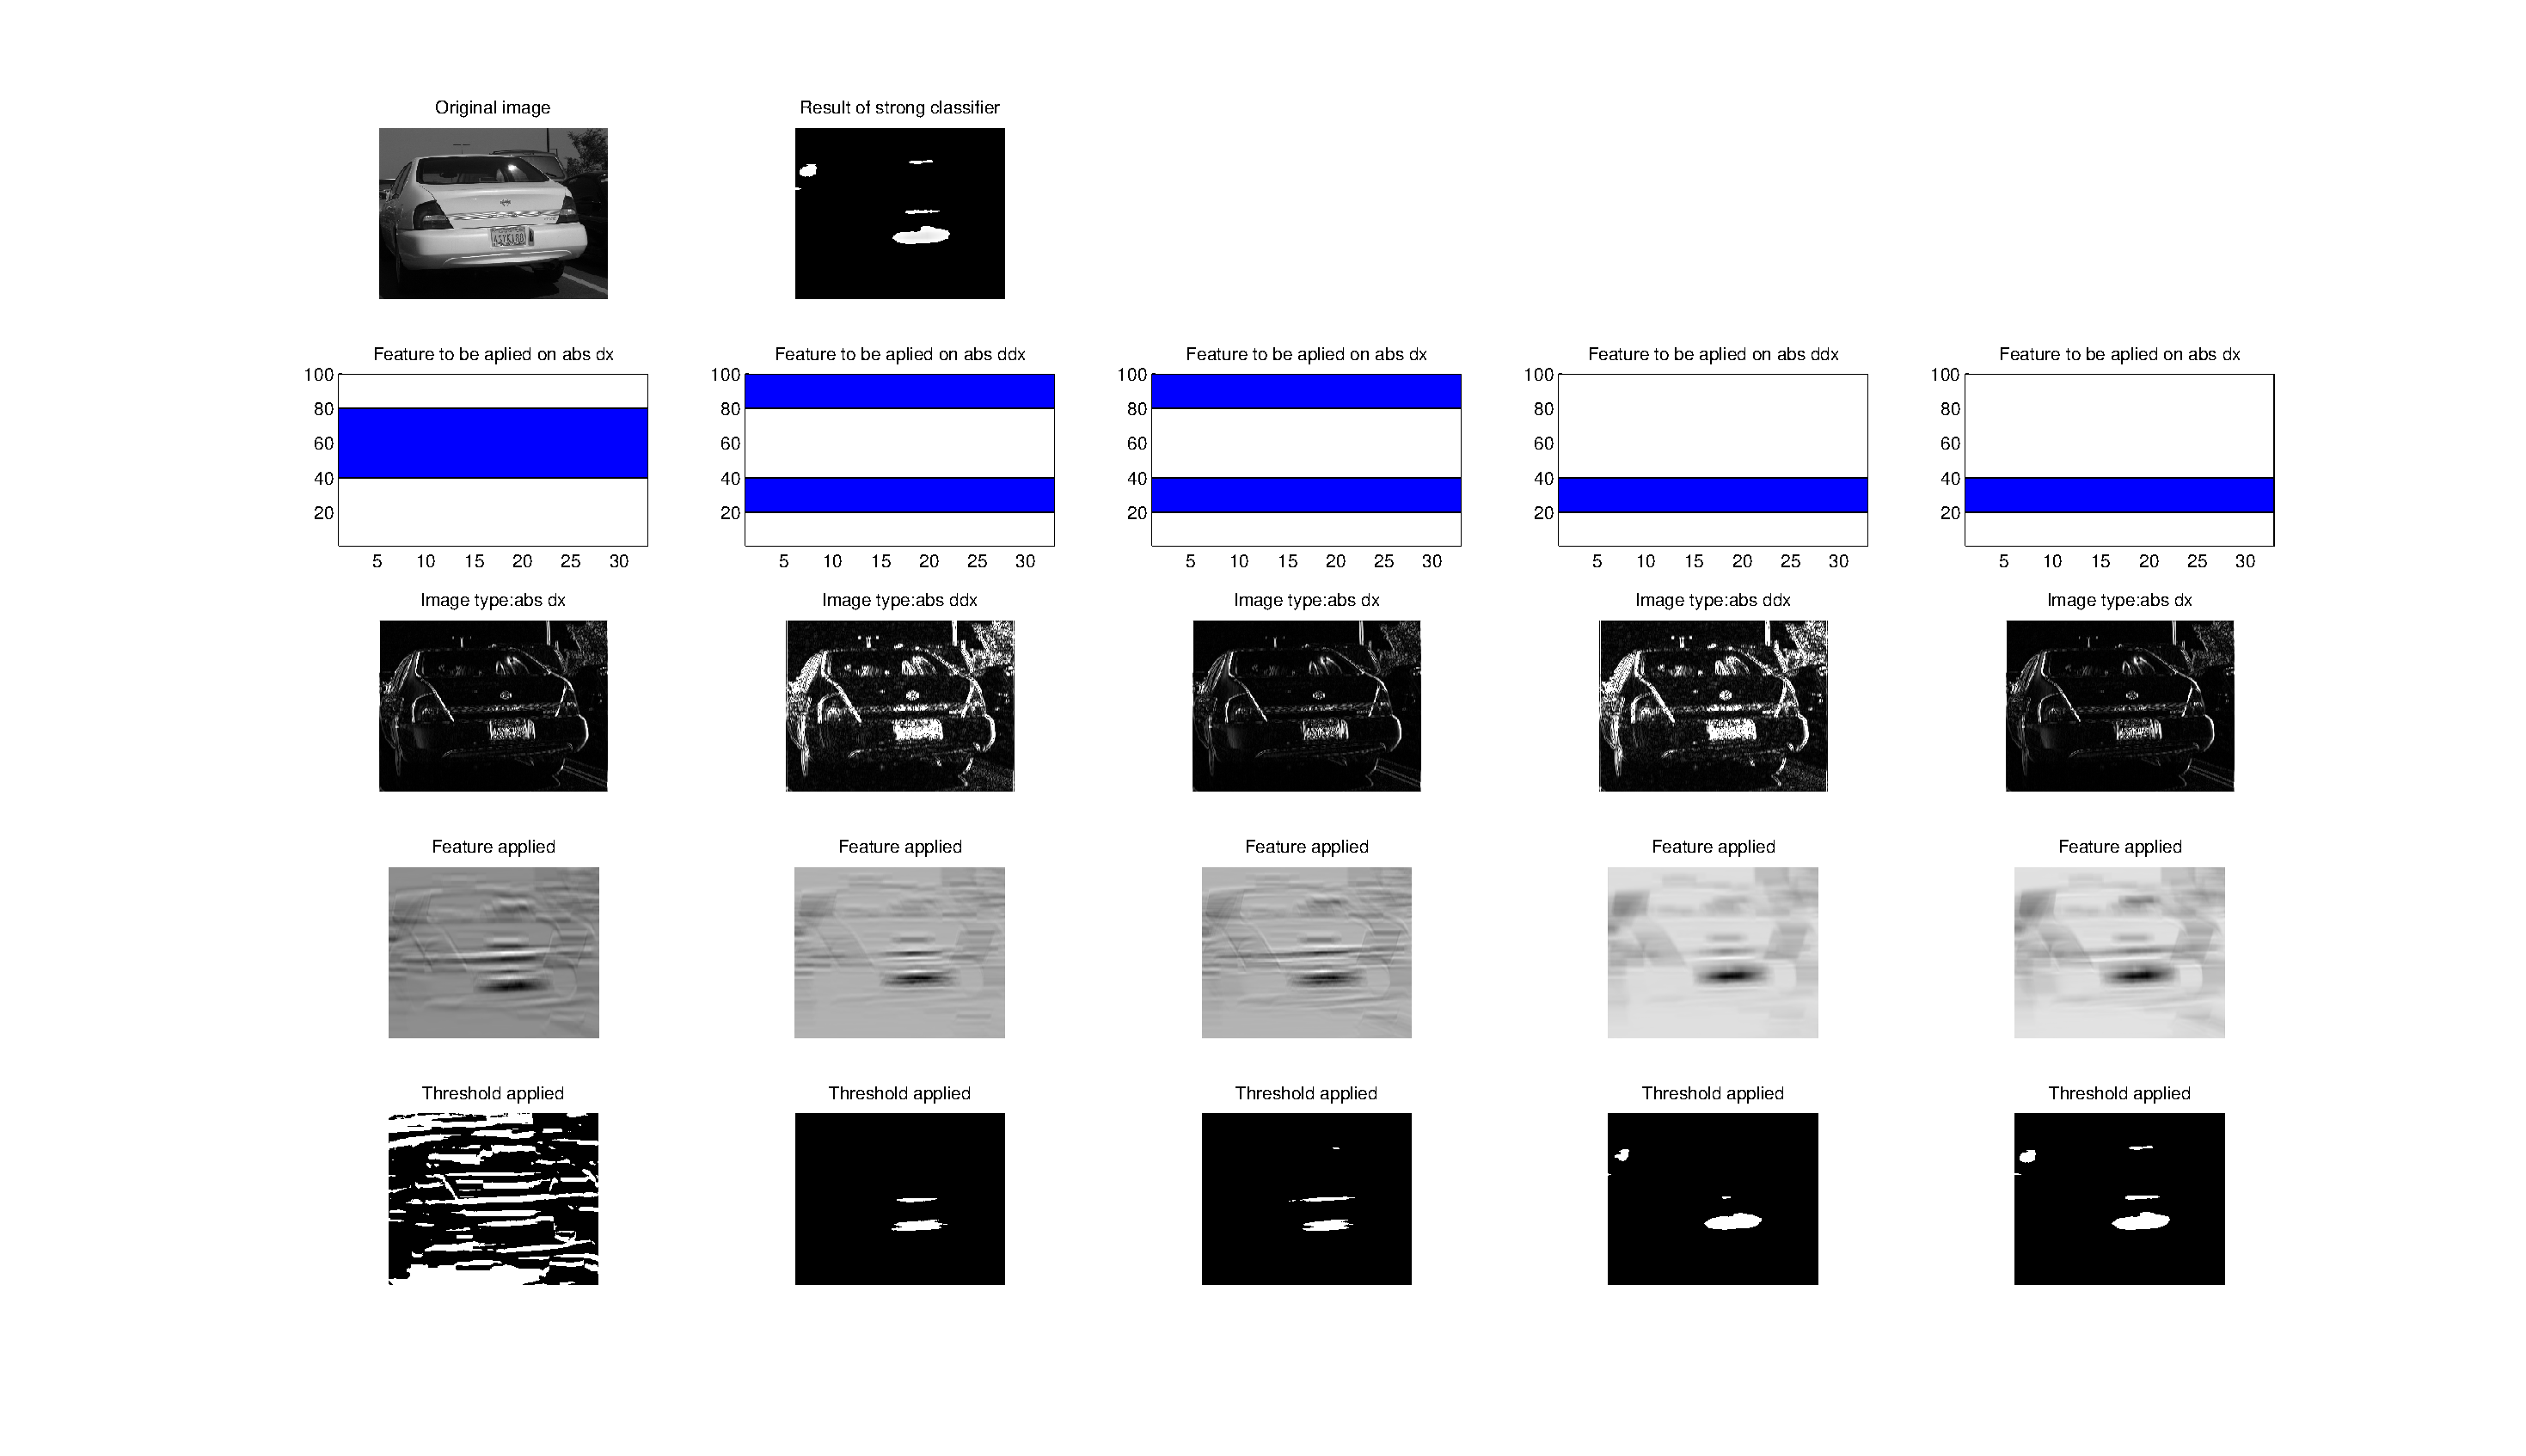
\includegraphics[width=10cm]{../report/img/strongClassifier_layer2_img14}
	\label{fig:strongclassify}
	\end{figure}
}

\section{Stage III: Cascading}
\frame
{
  \frametitle{Stage III: Cascading}
	
  \begin{itemize}
  \item <+-| alert@+> xxx
  \end{itemize}
}

\frame
{
	\begin{figure}[!ht]
	\centering
	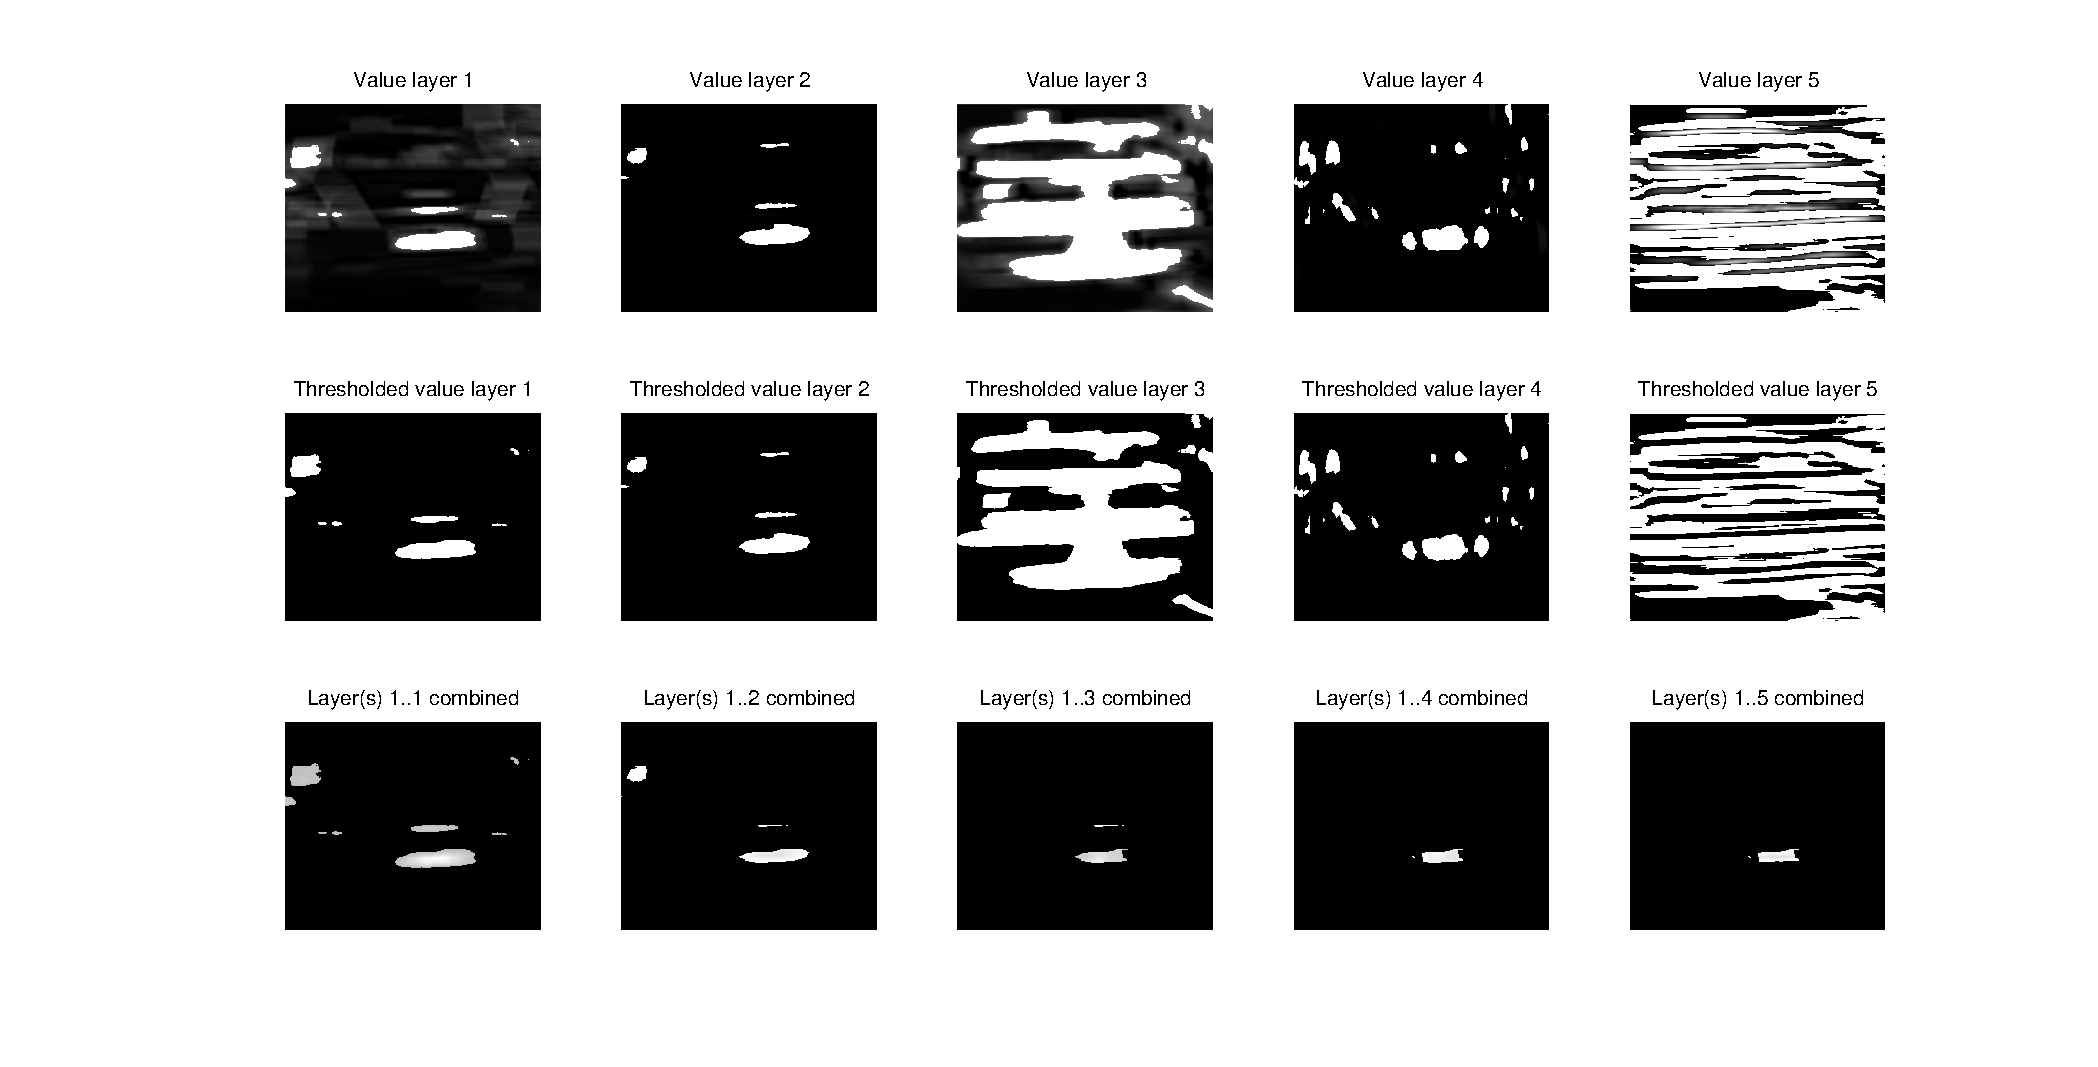
\includegraphics[width=12cm]{../report/img/cascader_img14}
	\label{fig:cascader}
	\end{figure}
}

\section{Results}
\frame
{
  \frametitle{Results}
	
  \begin{itemize}
  \item <+-| alert@+> xxx
  \end{itemize}
}

\frame
{
  \frametitle{Results}
	\begin{figure}[!ht]
	\centering

		\subfigure{
			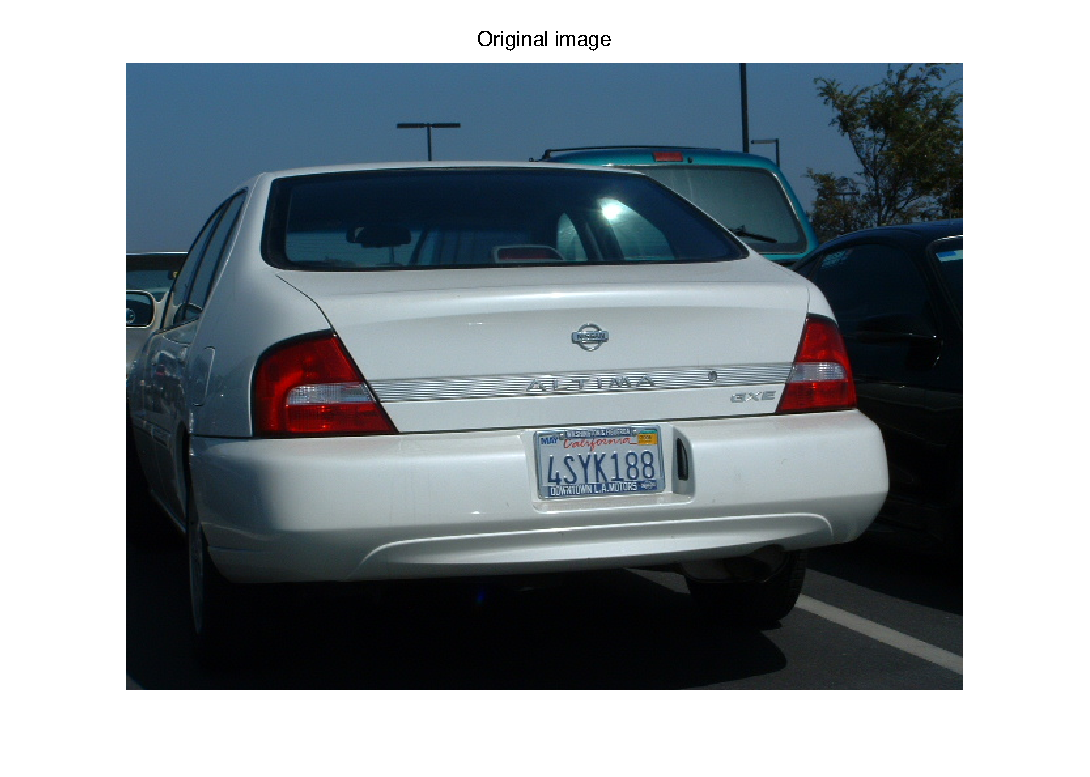
\includegraphics[width=5cm]{../report/img/cascader_original}
		}
		\subfigure{
			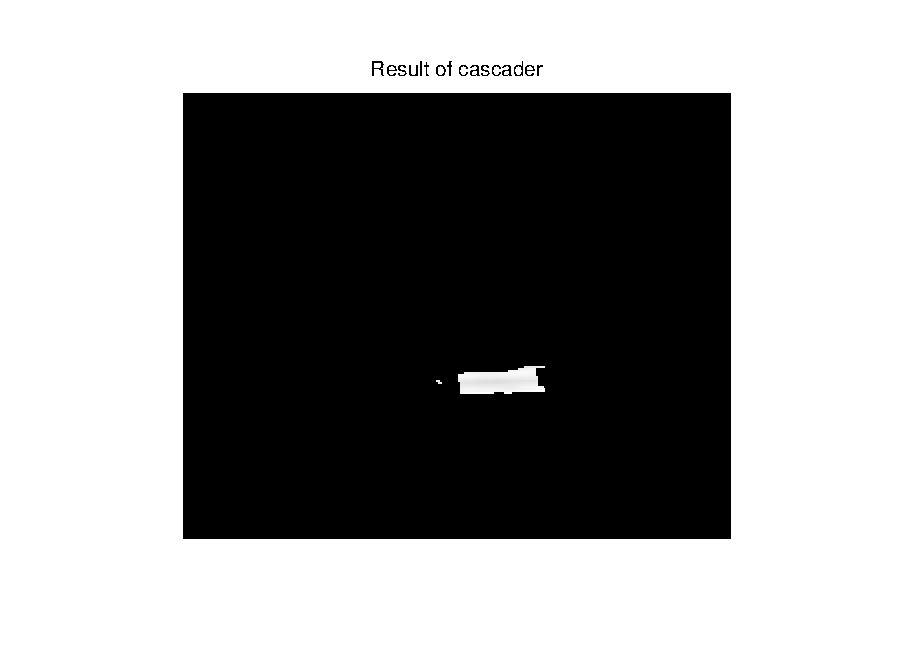
\includegraphics[width=5cm]{../report/img/cascader_result}
		}

	\end{figure}
}

\section{Conclusions}
\frame
{
  \frametitle{Conclusions}
	
  \begin{itemize}
  \item <+-| alert@+> xxx
  \end{itemize}
}

\AtBeginSection[]
{
 \begin{frame}
  \frametitle{Outline}
  \small
  \tableofcontents[currentsection,hideothersubsections]
  \normalsize
 \end{frame}
}

\end{document}
